\section{Factorial Design $2^2$}
\subsection{Theory}
\begin{frame}{Factorial Design $\pmb{2^2}$}
\framesubtitle{Problem Definition}

\begin{multicols}{2}
\textbf{Problem}
\begin{itemize}
    \item Two factors with two possible levels. \pause
    \item Simulation model.\pause
    \item It's desired to change a result of the simulation.
\end{itemize}

\columnbreak
\pause
\textbf{Objective}\\ \vspace{0.1cm} Analyze the effect that the factors have in the output of the model.
\end{multicols}
\pause
\begin{multicols}{2}
\textbf{Notation}
\begin{itemize}
    \item $n \rightarrow$ number of runs per treatment.
    \item $y_{i\lambda} \rightarrow$ output of $i^{\text{th}}$ simulation for the $\lambda^{\text{th}}$ treatment. 
    \item For each treatment $\lambda := \sum_{i=1}^n y_{i\lambda}$
\end{itemize}

\columnbreak
\centering
\textbf{Yates notation}
\begin{table}[]
\centering
\begin{tabular}{ccc}
\hline
      & Factor $A$ & Factor $B$ \\ \hline
$(1)$ & Low        & Low        \\
$a$   & High       & Low        \\
$b$   & Low        & High       \\
$ab$  & High       & High       \\ \hline
\end{tabular}
\label{tab:yates}
\end{table}
\end{multicols}
\end{frame}

\begin{frame}{Factorial Design $\pmb{2^2}$}
\framesubtitle{Workflow}
\begin{multicols}{2}
\onslide<2->{\textbf{Contrasts}\\
\begin{table}[H]
\centering
\begin{tabular}{lccc}
\hline
      & \multicolumn{1}{l}{Cont $A$} & \multicolumn{1}{l}{Cont $B$} & \multicolumn{1}{l}{Cont $AB$} \\ \hline
$(1)$ & -                                & -                                & +                                 \\
$a$   & +                                & -                                & -                                 \\
$b$   & -                                & +                                & -                                 \\
$ab$  & +                                & +                                & +                                 \\ \hline
\end{tabular}
\label{tab:contrast}
\end{table}}
\onslide<3->{
Equations:
$$\begin{array}{l}{\text { Cont } A=[a+a b-b-(1)]} \\ {\text { Cont } B=[b+a b-a-(1)]} \\ {\text { Cont } A B=[a b+(1)-a-b]}\end{array}$$
}
\onslide<4->{
\textbf{Effects}
\begin{equation*}
    \text{Effect } \chi = \dfrac{\text{Cont } \chi}{2n}, \quad \chi = A, B, AB
\end{equation*}}
\columnbreak
\onslide<1->{
\begin{figure}
    \centering
    \only<1>{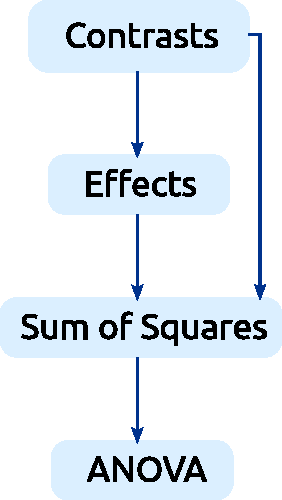
\includegraphics[scale=0.6]{images/proc.pdf}}
    \only<2>{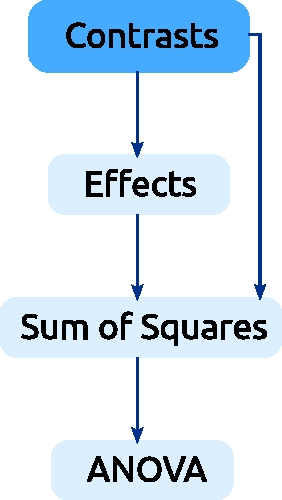
\includegraphics[scale=0.6]{images/contrast.pdf}}
    \only<3>{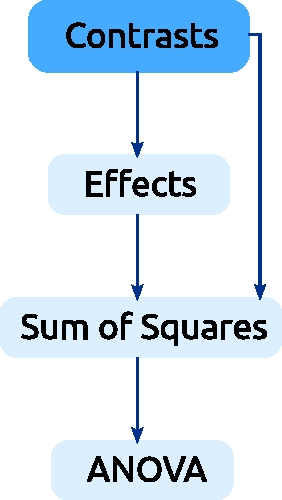
\includegraphics[scale=0.6]{images/contrast.pdf}}
    \only<4>{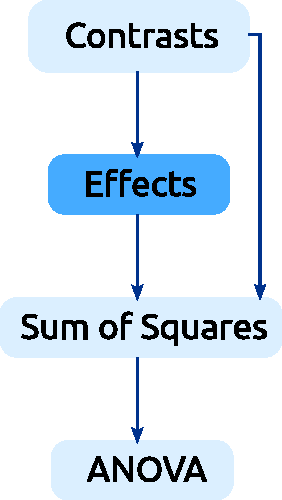
\includegraphics[scale=0.6]{images/effects.pdf}}
\end{figure}}
\end{multicols}
\end{frame}

\begin{frame}{Factorial Design $\pmb{2^2}$}
\framesubtitle{Workflow}
\begin{multicols}{2}
\onslide<1->{
\textbf{Squared sum}
\begin{equation*}
    \begin{split}
    \text{SS}_{\chi} =& \dfrac{(\text{Cont }\chi)^2}{2^2n},  \quad \text{df}_\chi = 1\\
    \text{SS}_t =& \sum_\lambda \sum_{i=1}^n y_{i\lambda}^2 -
    \dfrac{y_{..}^2}{2^2n},\quad \text{df}_t=2^2n-1\\
    \text{SS}_e =& \text{SS}_t - \sum_\chi \text{SS}_\chi, \quad \text{df}_e = 2^2(n-1)
    \end{split}
\end{equation*}
\onslide<2->{ 
\textbf{Average Squares:}
\begin{equation*}
    \text{AS}_\beta=\dfrac{\text{SS}_\beta}{df_\beta}
\end{equation*}}
}
\columnbreak
\onslide<1->{
\begin{figure}
    \centering
    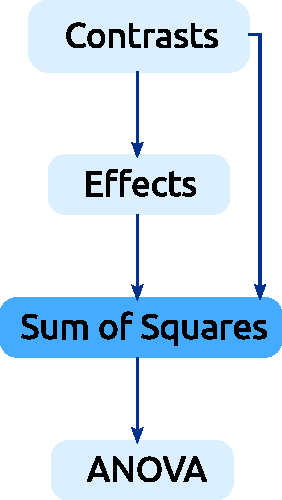
\includegraphics[scale=0.6]{images/sum.pdf}
\end{figure}}
\end{multicols}
\end{frame}


\begin{frame}{Factorial Design $\pmb{2^2}$}
\framesubtitle{Workflow}\begin{multicols}{2}
\textbf{ANOVA:}\\\vspace{0.5cm} 
$H_0:$ Effect A $ =0$\\ \vspace{0.3cm}
$H_0:$ Effect B $   =0$\\\vspace{0.3cm} 
$H_0:$ Effect AB $ =0$\\\vspace{0.5cm} 

Test:
\begin{align*}
    F_{0\chi} &= \dfrac{\text{AS}_{\chi}}{\text{AS}_e}, \quad F \sim \mathbb{F}_{(1,2^2(n-1))}\\ \vspace{0.5cm}
    P_{0\chi} &= \mathrm{P}(F>F_{0\chi})\\\vspace{0.5cm}
\end{align*}
Given a significance level $\alpha$, the null hypothesis ($H_0$) is rejected if $P_{0\chi} < \alpha$
\columnbreak
\begin{figure}
    \centering
    \centerline{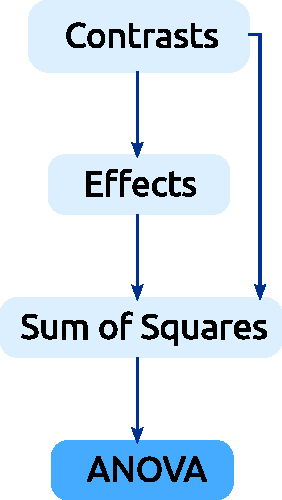
\includegraphics[scale=0.6]{images/anoa.pdf}}
\end{figure}
\end{multicols} 
\end{frame}

\subsection{Example}
\begin{frame}{Factorial Design $\pmb{2^2}$}
\framesubtitle{Example}
    Joe’s parlour is open from 9.00am to 7.00pm and he and his fitters work throughout that period if there is work to be done. Motorists arrive and wait for Joe to inspect their car’s exhaust system.Joe drives the car onto any free hydraulic ramp for inspection.Joe then advises the customer on the necessary work and customers elect to stay or go off elsewhere. When the fitter is finished, Joe inspects the work and, if satisfactory, he prints out the bill for the driver, who then pays and leaves. If Joe decides that the work is not satisfactory  then the fitter must rework the job – and this may take as long as the original work. 
    
    Joe would like some advice from you. He needs to know how many fitters and ramps he should employ in the parlour (currently, three ramps and two fitters) \citep{pidd1998computer}.
\end{frame}